The first step in designing a PCB is capturing the entire circuit schematic.  A circuit schematic was developed based on the designs for the Electrophysiology Interface board in section~\ref{sec:hardware} and can be seen in appendix~\ref{sec:schematic} on page~\pageref{sec:schematic}.  The schematic capture program of the KiCad EDA suite, Eeschema, handles complex, multi-sheet schematics with a hierarchical structure.

The root sheet of the schematic on page~\pageref{SchematicRev1r0.1} contains most of the input and output connectors, such as the Hirose FX2 connector, which marries the Electrophysiology Interface board to the RTSC board, and the terminal blocks for connecting to the biological electrodes, allowing the overall signal flow to be summarized on one sheet.  To add more sheets to the design, a block is added to the root sheet representing the sheet added to the design hierarchy and referencing a schematic file that defines the contents of the sheet.  Figure~\ref{fig:hblock} shows a hierarchical block on the root sheet that adds the sheet, PreAmpInterface, found on page~\pageref{SchematicRev1r0.2}, to the design hierarchy with its contents pulled from the file, PreAmpInterface.sch, in the project directory.

\begin{figure}[h]
	\begin{singlespace}
	\centering
%	\setlength\fboxsep{0pt}
%	\setlength\fboxrule{0.5pt}
%	\fbox{ }
	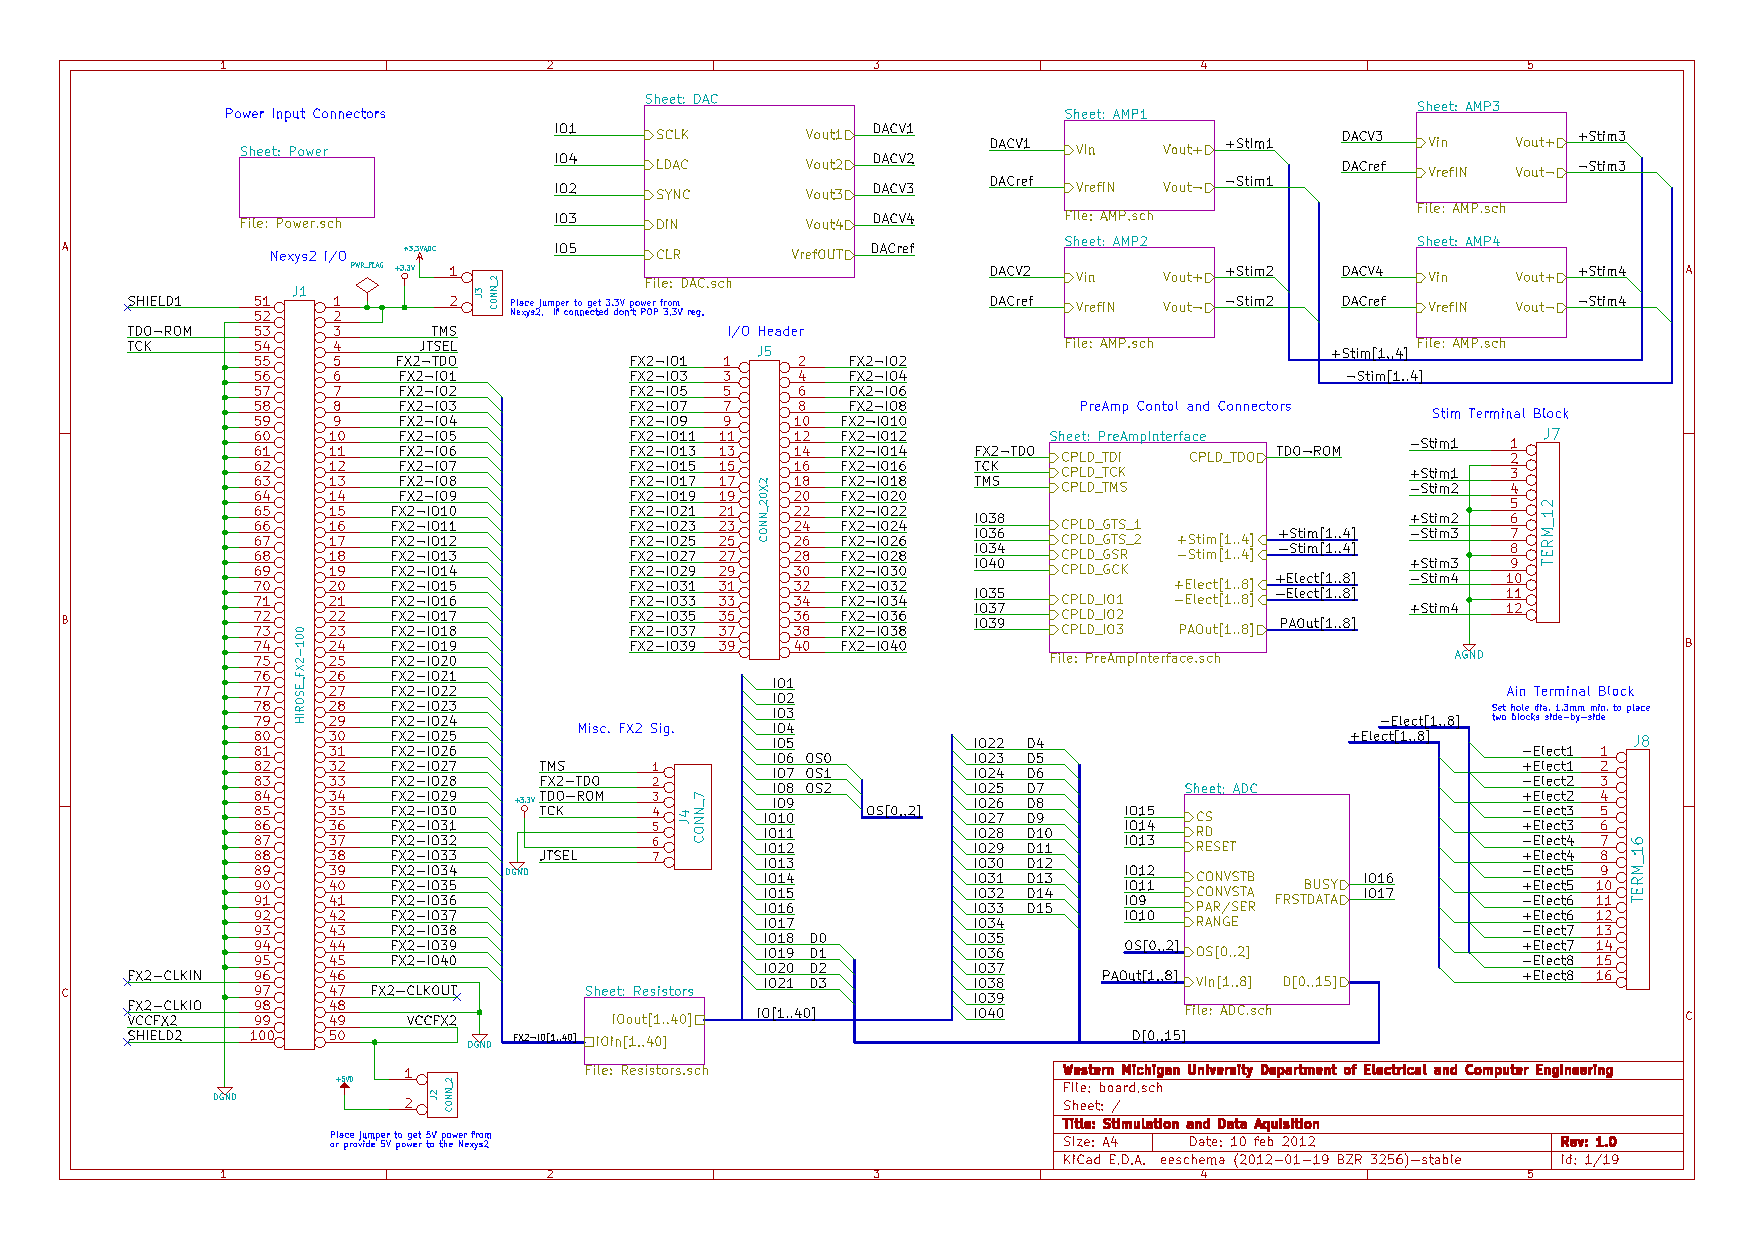
\includegraphics[page=1,trim=6.4in 3.7in 2.6in 2.8in,clip]{./figures/SchematicRev1r0} %[trim=left bottom right top]
	\caption{Example of a hierarchical block used to add sheets to the schematic\label{fig:hblock}}
	\end{singlespace}
\end{figure}

Local net labels, such as TCK on the root sheet, connect signals with the same net label without the need to draw a wire but are only valid on the same sheet.  Any signal labeled TCK on another sheet will not be connected the net on the root sheet.  To connect signals between sheets, hierarchical labels may be included on the sheet.  A hierarchical label, such as CPLD\_TCK on the PreAmpInterface sheet, is similar to a local net label in that its scope is only within the sheet but is special in that it can appear on the block symbol for the sheet.  Connecting a signal to the label on the block symbol connects the signal to the net designated by the hierarchical label, such as the TCK net on the root sheet connecting to the CPLD\_TCK net on the PreAmpInterface sheet by virtue of the connection of TCK to CPLD\_TCK on the block shown in Figure~\ref{fig:hblock}.

Hierarchical blocks can be called from any sheet in the hierarchy, not just the root sheet, which allows for multi-level hierarchies.  Figure~\ref{fig:hierarchy} shows the hierarchical structure of the Electrophysiology Interface board schematic.  Most blocks are called from the root sheet with the exception of the PreAmpInterface sheet, which itself calls several blocks.

\begin{figure}[h]
	\begin{singlespace}
	\centering
	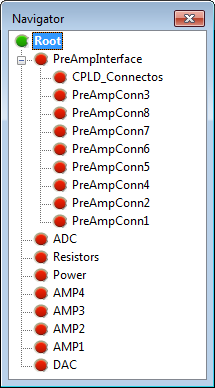
\includegraphics[width=1.5in]{./figures/Hierarchy}
	\caption{Sheet hierarchy in the Electrophysiology Interface board schematic \label{fig:hierarchy}}
	\end{singlespace}
\end{figure}

One of the advantages of hierarchical blocks is that, when parts of the circuit need to be replicated, such as in the case of the Differential Output Amplifier described in section~\ref{sec:DOA}, only one iteration of the circuit needs to be drawn.  Multiple hierarchical block symbols can reference a single schematic file.  Any changes to the circuit in one sheet will propagate to the other sheets whose blocks reference the same schematic file.  Figure~\ref{fig:hblockx4} shows how one schematic file is referenced by multiple blocks to allow four Differential Output Amplifier circuit blocks to be included in the schematic while only being drawn once.

\begin{figure}[h]
	\begin{singlespace}
	\centering
	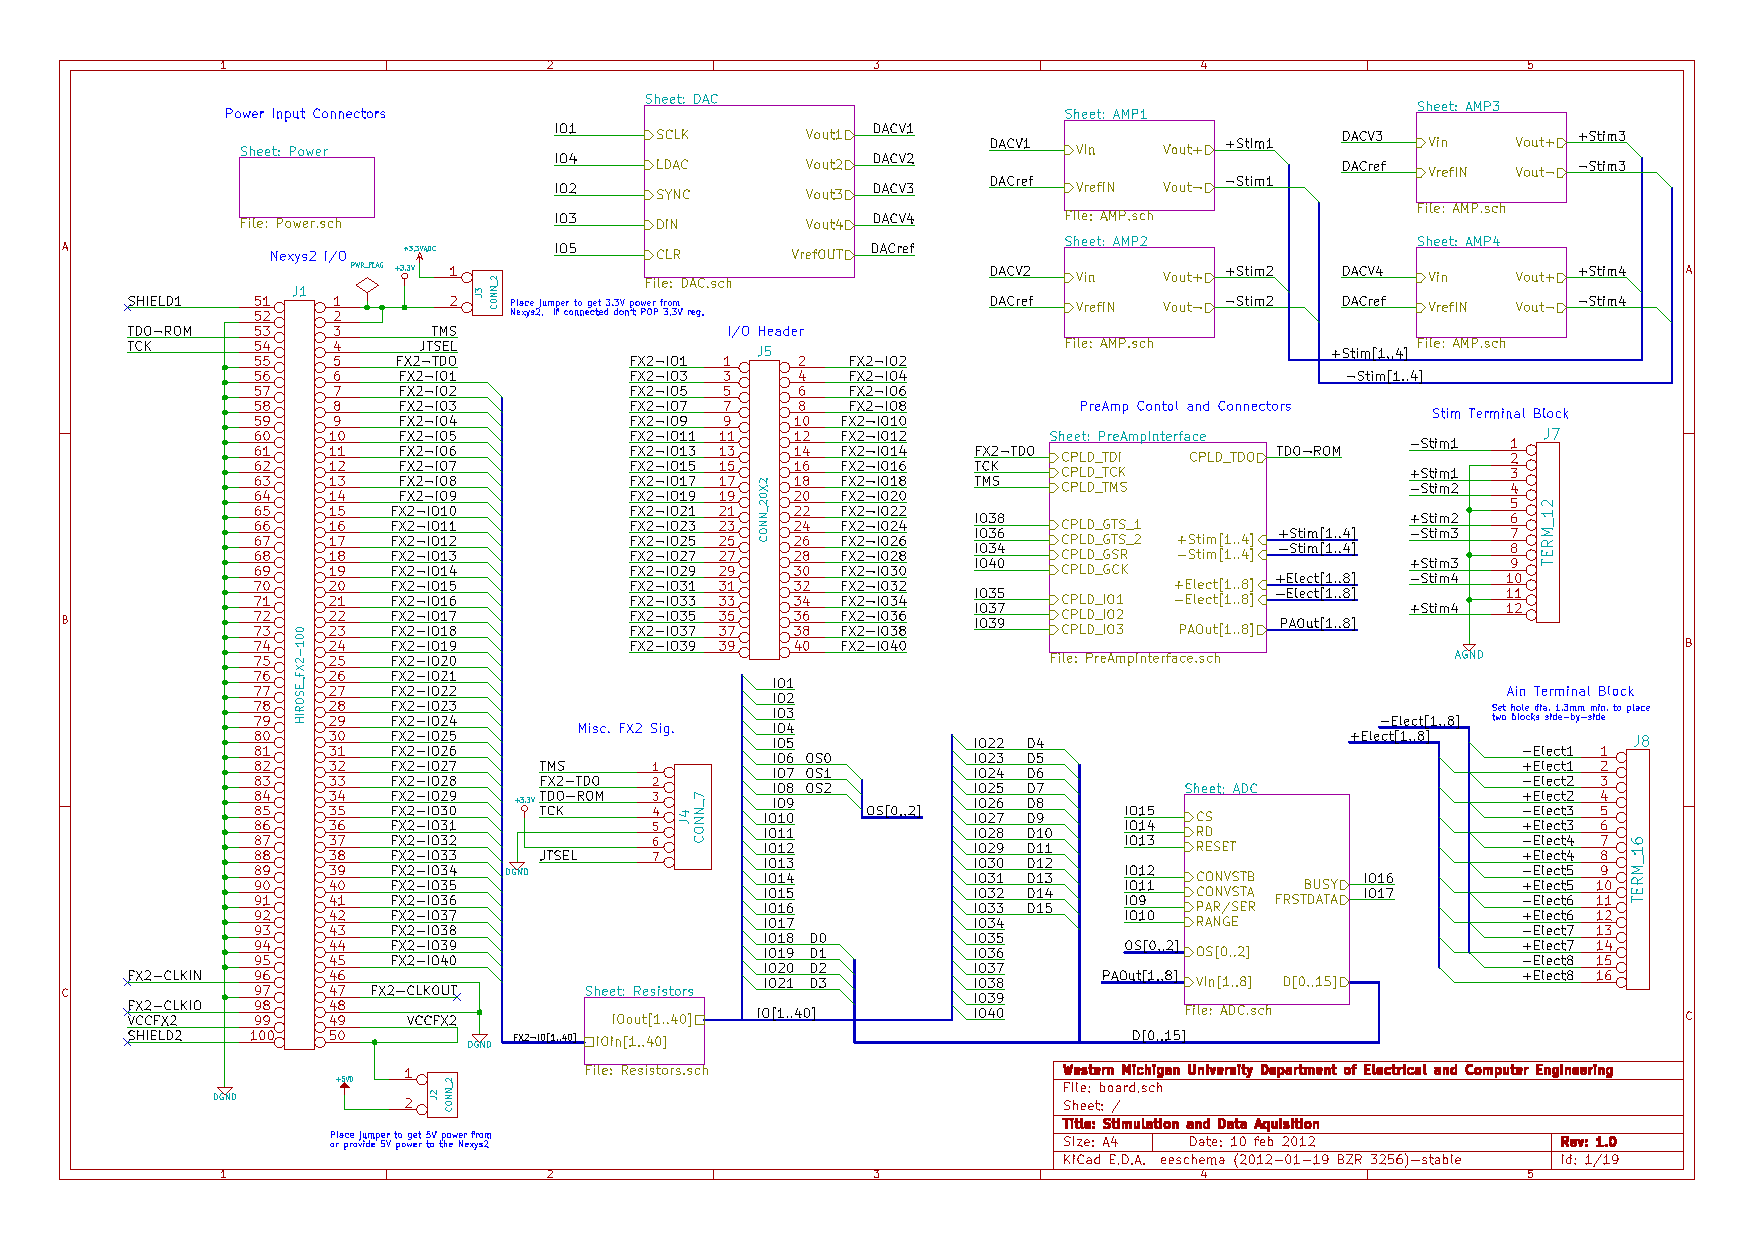
\includegraphics[page=1,trim=6.5in 5.6in 0.5in 0.6in,clip]{./figures/SchematicRev1r0} %[trim=left bottom right top]
	\caption{An example of four hierarchical blocks being used to replicate a single circuit design \label{fig:hblockx4}}
	\end{singlespace}
\end{figure}

The sheets AMP4 down to AMP1 on pages~\pageref{SchematicRev1r0.15} to~\pageref{SchematicRev1r0.18} are nearly identical, but it should be noted that the reference designators of the components on each sheet are unique.  For instance, the decoupling capacitors on sheet AMP1 are labeled C24 and C25 while the decoupling capacitors on sheet AMP2 are labeled C22 and C23.  Changing a reference designator on one sheet will not affect the other sheets, but adding or deleting components or drawing wires on one sheet will propagate to the other sheets.

Multiple component symbols are custom made for the Electrophysiology Interface board.  Most are based on symbols from KiCad symbol library and the information contained in the respective parts data sheets.  The Preamp PCI-Express connector symbol is based on a library from~\cite{osheclib}.  All custom component library files are stored in the $lib$ directory under the project directory to facilitate project portability between installations of KiCad.

Test points are included for most signals to facillitate rework and voltage measurement, with the exception of the CPLD and FPGA IO pins and JTAG signals, which are connected to header components.
